\documentclass[a4paper,14pt]{article}

\usepackage{etex} % расширение классического tex

% для русского языка
\usepackage{cmap}					% для поиска русских слов в pdf
\usepackage[12pt]{extsizes}			% нестандартные размеры шрифта
\usepackage[X2,T2A]{fontenc}		% кодирование шрифтов в pdf
\usepackage[utf8]{inputenc}			% задание utf8 кодировки исходного tex файла
\usepackage[english,russian]{babel}	% выбор языка для документа, локализация и переносы
\usepackage{setspace}				% пробелы
\usepackage{epigraph,csquotes}		% для эпиграфов и продвинутых цитат

\usepackage{sectsty}				% управление стилем секционирования
\allsectionsfont{\normalsize}
\subsectionfont{\normalsize\indent} 
\subsubsectionfont{\normalsize\indent\indent} 

\usepackage{verbatim}				% для многострочных комментариев
\usepackage{makeidx}				% для создания предметных указателей
\usepackage{indentfirst}			% установка отступа в первом абзаце главы

\usepackage{geometry} 				% меняем поля страницы
\geometry{left=1.5cm}				% левое поле
\geometry{right=2cm}				% правое поле
\geometry{top=1cm}					% верхнее поле
\geometry{bottom=2cm}				% нижнее поле

\usepackage{amsmath,amsfonts,amssymb,amsthm,mathtools} % математика
\usepackage{mathrsfs}				% торжественные буковки
\usepackage{bm, bbm}				% шрифты
\usepackage{wasysym}				% нестандартные символы
\usepackage{textcomp}				% чтобы в формулах можно было русские буквы писать через \text{}

\usepackage{enumerate}				% списки
\usepackage{enumitem}				% дополнительные плюшки для списков
\usepackage{float}
\usepackage{array}					% таблички
\usepackage{dcolumn}				% центрирование по разделителю для apsrtable
\usepackage{longtable}				% таблицы на несколько страниц
\usepackage{booktabs}				% красивые таблицы
\usepackage{multirow}
\usepackage[table,xcdraw]{xcolor}

\usepackage{graphicx}				% графика
\graphicspath{{images/}}			% путь к картинкам
\usepackage{subfigure}				% для создания нескольких рисунков внутри одного
\usepackage{caption}				% для организации подписей
\captionsetup{format=plain,justification=centerlast}

\usepackage{tikz,pgfplots}			% язык для рисования графики из latex'a
\usetikzlibrary{trees}				% tikz-прибамбас для рисовки деревьев
\usepackage{tikz-qtree}				% альтернативный tikz-прибамбас для рисовки деревьев
\usetikzlibrary{arrows}				% tikz-прибамбас для рисовки стрелочек подлиннее

\usepackage{color}					% цветные ссылки
\definecolor{downgrade}{rgb}{0.0, 0.5, 1.0}
\usepackage[pdfhighlight=/N,colorlinks=true,unicode,pdftex]{hyperref}% внутренние ссылки

\usepackage[labelsep=endash]{caption}		% кастомизация подписей в плавающих окружениях

% новая команда \RNumb для вывода римских цифр
\newcommand{\RNumb}[1]{\uppercase\expandafter{\romannumeral #1\relax}}

% нестандартные подписи
\addto\captionsrussian{\def\chaptername{Глава}}
\addto\captionsrussian{\def\contentsname{Содержание}}
\addto\captionsrussian{\def\listfigurename{Список рисунков}}
\addto\captionsrussian{\def\listtablename{Список таблиц}}
\addto\captionsrussian{\def\abstractname{Аннотация}}
\addto\captionsrussian{\def\refname{Список использованных источников}}
\addto\captionsrussian{\def\indexname{Предметный указатель}}
\addto\captionsrussian{\def\figurename{Рисунок}}
\addto\captionsrussian{\def\tablename{Таблица}}
\addto\captionsrussian{\def\partname{Часть}}
\addto\captionsrussian{\def\appendixname{Приложение}}

\usepackage{todonotes}				% для вставки в документ заметок о том, что осталось сделать
% \todo{Здесь надо коэффициенты исправить}
% \missingfigure{Здесь будет Последний день Помпеи}
% \listoftodos --- печатает все поставленные \todo'шки/
\author{Аксенова Светлана, Гарина Ольга}
\title{Лабораторная работа \\ Спектроскопия электронного парамагнитного резонанса}
\begin{document}
	\begin{titlepage}
		
		\begin{center}
			\vfill
			%\framepage
			
			Министерство образования Российской Федерации\\
			Московский физико-технический институт (национальный исследовательский университет)\\
			\ \\
			\hfill
			
			\vfill
		
			
			{\large\bf Спектроскопия электронного парамагнитного резонанса\\}
			\ \\
		Лабораторная работа студентов группы Б04-901 \\
			Аксеновой Светланы\\
			Гариной Ольги
			
			\vfill
			
			
			
			\vfill
			
			Долгопрудный, 2022
		\end{center}
		
	\end{titlepage}
	\newpage
	\tableofcontents	
	\newpage
\textbf{Цель лабораторной работы}: исследование
сверхтонкой структуры спектров электронного парамагнитного резонанса (ЭПР), измерение скорости спин-спинового обмена в растворах и кристаллах, исследование влияния амплитуды высокочастотной модуляции и уровня диэлектрических потерь на вид спектров ЭПР.
\par 
Метод электронного парамагнитного резонанса применяется для исследования парамагнитных центров и их окружения в веществе. Методом ЭПР можно определять концентрацию и идентифицировать парамагнитные частицы в любом агрегатном состоянии. Он позволяет детектировать свободные радикалы в количестве до $ 10^{-10} - 10^{-13} $ М.
\section{Физические основы спектроскопии ЭПР}
Атомы и молекулы, имеющие незаполненную электронную оболочку, обладают электронными магнитными моментами $ \mathbf{\mu} $ даже в отсутствие внешнего магнитного поля. Для веществ, состоящих из таких частиц, наблюдаются парамагнитные свойства. Во внешнем магнитном поле уровни энергии парамагнитной частицы расщепляются на дискретные подуровни:
\begin{equation}
	E=-(\mathbf{\mu}, \mbox{\boldmath$H_0$})=g \beta H_0 m_J,
\end{equation}
где $ \beta = e\hbar/2mc $ - магнетон Бора, $ m_J $ - магнитное квантовое число, а $ g $ - фактор спектроскопического расщепления.
\par 
Под действием электромагнитного излучения будут происходить переходы между такими уровнями (рис. 1), если энергия кванта излучения близка к разнице энергий между ними и соблюдается правило отбора по магнитному квантовому числу $ \Delta m_J = \pm 1 $:
\begin{equation}
	h \nu = \Delta E = g \beta H_0.
\end{equation}
\begin{figure}[h]
	\centering
	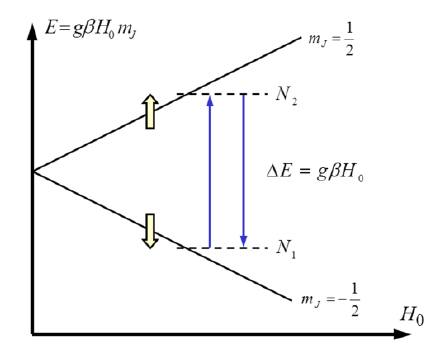
\includegraphics{рис1}
	\caption{Энергетические уровни электрона во внешнем магнитном поле $ H_0 $}
	\label{fig:1}
\end{figure}
\par 
В стационарном состоянии на более низких по энергии уровнях находятся несколько больше частиц  $ N_1 > N_2 $, а вероятность переходов $ w_{1\rightarrow2}=w_{2\rightarrow1}, в итоге будут преобладать переходы снизу вверх $  $ 1\rightarrow2 $	(рис. 1), т.е. с поглощением энергии излучения. Избирательное поглощение энергии системой парамагнитных частиц при определенном отношении напряженности постоянного магнитного поля к частоте радиоизлучения получило название электронного парамагнитного резонанса.
\subsection{Квантовомеханическое рассмотрение ЭПР}
Уровни энергии электрона, вырожденные по проекции спина, расщепляются на два подуровня. Величина расщепления определяется значением внешнего магнитного поля $ H_0 $. 
\par 
Орбитальному движению электронов соответствует магнитный момент, проекцию которого можно выразить через гиромагнитное соотношение:
\begin{equation}
	\mu_z=\gamma l_z = -\frac{e}{2mc}\hbar m_l.
\end{equation}
Проекцию магнитного момента принято писать в виде
\begin{equation}
	\mu_z = -g_l \beta m_l,
\end{equation}
где $ g_l = 1$ - g-фактор орбитального движения электрона.  
\par 
Опыт показывает, что для многих парамагнитных частиц значение g-фактора близко к 2. Это связано с тем, что электрон обладает также собственным механическим моментом (спином) и собственным магнитным моментом.
\par 
Если атомная частица содержит несколько электронов, то их орбитальные и спиновые моменты складываются, так для связи Рассела-Саундерса: $ \mathbf{L}=\Sigma \mathbf{l_i} $, $ \mathbf{S}=\Sigma \mathbf{s_i} $. Полный механический момент частицы $ \mathbf{J=L+S} $ складывается из её спинового и орбитального моментов, аналогично формируется и полный магнитный дипольный момент. Величина g-фактора будет отличаться от чисто спинового или орбитального значений (для него справедлива формула Ланде). 
\par 
Спиновый и орбитальный магнитные моменты электрона взаимодействуют между собой (спин-орбитальное взаимодействие). Это приводит к отклонению величин g-факторов радикалов от чисто спинового значения $ g_s $:
\begin{equation}
	g=g_s \left(1-\frac{a \lambda_{SL}}{\Delta E}\right),
\end{equation}
где $ \Delta E $ - расщепление между основным и ближайшим по энергии орбитальным состоянием, участвующим в орбитальном движении; $ a $ - множитель, который зависит от природы парамагнитного центра и ориентации его по отношению к внешнему магнитному полю. Энергия спин-орбитального взаимодействия $ E=\lambda_{SL}(\mathbf{S \cdot L}) $ может быть охарактеризована некоторым усредненным числовым коэффициентом - константой спин-орбитального взаимодействия: $ |\lambda_{SL}| \approx 10^{-5} \div 10^{-2}$ эВ. 
\subsection{Сверхтонкая структура линий спектров ЭПР}
Если ядро атома также обладает магнитным моментом (имеет ненулевой спин), структура линий ЭПР спектра становится более сложной.
\par
При достаточно больших внешних полях ($ H_0 > 10-100 $ Э) энергия взаимодействия магнитного момента электронной оболочки с этим полем будет больше, чем энергия взаимодействия с магнитным моментом ядра. Это приведет к <<разрыву>> связи ядра и электронной оболочки, т.е. магнитные моменты ядра и электронной оболочки будут ориентироваться во внешнем магнитном поле независимо друг от друга. Такое взаимодействие магнитных моментов электрона и ядра приводит к изменению условия резонанса и носит название сверхтонкого взаимодействия (СТВ).
\par 
 Для ядра, имеющего спин $ I $, возможны $ 2I + 1 $ различных ориентаций. Энергии ядер в этих ориентациях будут различаться на величину $ g_{\text{яд}}\beta_{\text{яд}}H_0 $. Эти различия малы по сравнению с тепловой энергией, поэтому можно считать, что равновесные заселенности уровней, соответствующие различным ориентациям ядер, одинаковы. Тогда электроны различных атомов будут находиться в локальных магнитных полях, создаваемых ядрами, имеющих $ 2I + 1 $ различных значений. Условие резонанса при плавном изменении внешнего магнитного поля будет выполняться для электронов $ 2I + 1 $ раз, т.е. произойдет расщепление линии поглощения (образование сверхтонкой структуры ЭПР атома водорода показано на рис. 2). Расстояние между линиями сверхтонкой структуры называется константой сверхтонкого взаимодействия ($ a $).
\begin{figure}[h]
	\centering
	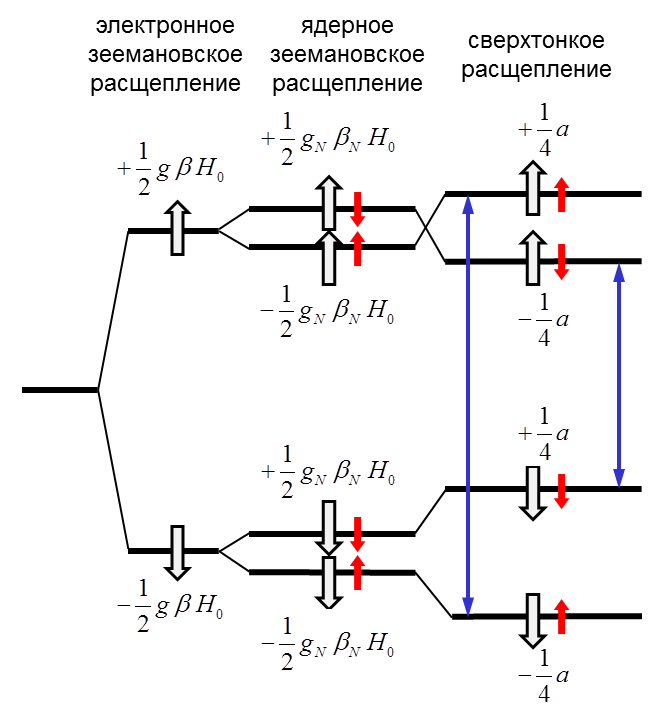
\includegraphics{рис2}
	\caption{Образование сверхтонкой структуры спектра ЭПР атома водорода}
	\label{fig:2}
\end{figure}
\par 
Характерным признаком для расщепления линий в спектре ЭПР под
влиянием парамагнитных ядер одиночных атомов является равная
интенсивность всех линий.
\par 
В том случае, когда мы имеем дело с многоатомным радикалом c
суммарным спином $ S = 1/2 $, локальное магнитное поле будет определяться суммарным действием нескольких близлежащих магнитных ядер $ \{i\} $.
\par 
Правила отбора для переходов, возбуждаемых при ЭПР: $ \Delta m_S = \pm1 $, $ \Delta m_i = 0 $, что соответствует закону сохранения момента импульса при взаимодействии магнитного дипольного фотона (со спином 1) с электроном.
\subsection{Уширение линий и релаксационные процессы}
Ширина линии поглощения $ \delta \omega $ и ширина уровня энергии $ \delta E $ связаны со временем жизни частицы на определенном уровне энергии $ \tau $ соотношением неопределенностей:
\begin{equation}
	\delta \omega \cdot \tau \backsim 1 \text{ или } \delta E \cdot \tau \backsim \hbar.
\end{equation}
\par 
Время жизни $ \tau $ определяется релаксационными процессами, происходящими при взаимодействии спинов друг с другом и с другими степенями свободы системы. Существует два типа релаксационных процессов: продольная (релаксация продольной намагниченности образца к её равновесному значению вдоль внешнего постоянного магнитного поля, энергия спиной системы изменяется) и поперечная релаксация (обнуление поперечных компонент вектора намагниченности образца, энергия не изменяется). В процессе поперечной релаксации происходит расфазировка прецессии магнитных моментов, которая обусловлена как различием частот прецессии векторов намагниченности в неоднородном магнитном поле, так и спин-спиновой релаксацией, при которой взаимодействие двух частиц приводит к изменению спиновых состояний каждой из них.
\par 
Время поперечной релаксации меньше времени продольной, поэтому оно ограничивает время жизни спинового состояния и определяет ширину резонансных линий $ \delta \omega $. Времена релаксации и связанная с ними ширина линий поглощения могут изменяться при изменении параметров изучаемой системы.
\par 
Главный вклад в ширину линии вносят релаксационные процессы, связанные со спин-спиновым взаимодействием. Уширение линий за счет спин-спинового взаимодействия может быть уменьшено путем уменьшения концентрации парамагнитных частиц. Скорость спинового обмена $ 1/\tau_e $ пропорциональна частоте двойных соударений, т.е. пропорциональна концентрации $ C $ парамагнитных частиц в растворе:
\begin{equation}
	\frac{1}{\tau_e}=K_e C,
\end{equation}
где $ K_e $ - константа спинового обмена. В результате обмена спин электрона может оказаться в другом магнитном окружении.
\par
В случае медленного обмена расщепление линии на отдельные компоненты сохранится (рис. 3 А, Б), но при этом сократится время пребывания электрона в состоянии с тем или иным магнитным окружением. В соответствии с соотношением неопределенности это приведет к уширению каждой из компонент расщепленной линии:
\begin{equation}
	\delta H_e = \frac{1}{\gamma \tau_e}=K_e C \frac{1}{\gamma}.
\end{equation}
При быстром обмене локальное магнитное поле усредняется. В спектре при этом наблюдается только одна линия резонанса - на средней частоте (рис. 3В), т.к. электронных спин, фактически, находится в усреднённом магнитном поле, поэтому резонансные линии в спектре становятся более узкими (обменное сужение).
\begin{figure}[h]
	\centering
	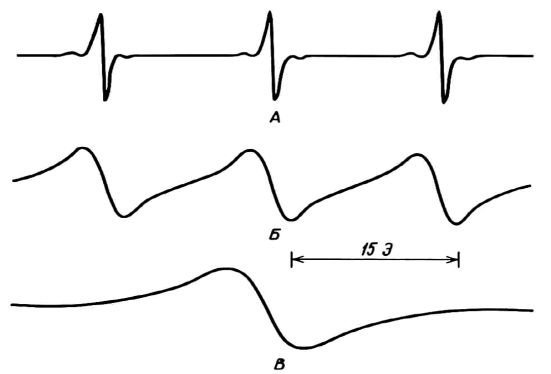
\includegraphics{рис3}
	\caption{ЭПР спектр растворов радикала $ \mathrm{[(CH_3)_3C]_2NO} $ в случае медленного (А, Б) и быстрого (В) спинового обмена. Концентрации радикала: А – $ 10^{-4} $ М; Б – $ 10^{-2} $ М; В – 10$^ {-1} $ М}
	\label{fig:3}
\end{figure}
\section{Экспериментальная установка}
Основными компонентами любого спектрометра ЭПР в микроволновом диапазоне являются:
\begin{itemize}
	\item постоянный магнит (или магнитная система);
	\item генератор СВЧ излучения;
	\item резонатор с местом для введения образца;
	\item детектор СВЧ излучения;
	\item усилители сигнала;
	\item большинство ЭПР-спектрометров оборудованы также системой высокочастотной (ВЧ) модуляции сигнала.
\end{itemize}
На практике большинство спектрометров ЭПР работают либо на частоте 9 ГГц, соответствующей длине волны 3.2 см (Х-диапазон) и полю $ H_0 \backsim $ 3000 Э (при $ g $ = 2 – как у свободного электрона), либо на частоте 36 ГГц, соответствующей длине волны 8 мм (Q-диапазон). 
\begin{figure}[h]
	\centering
	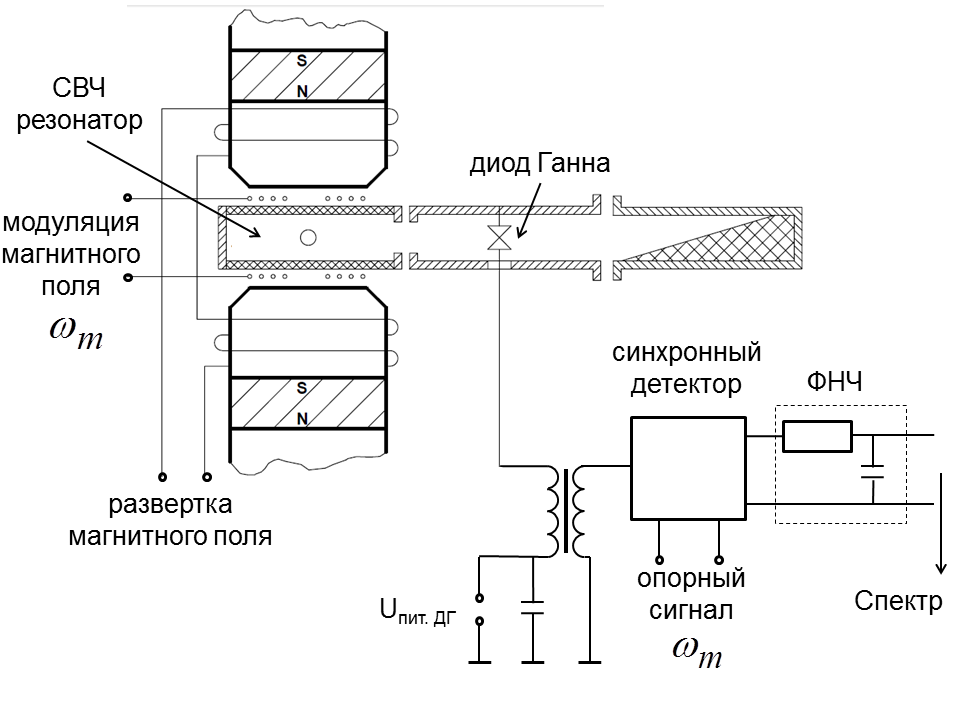
\includegraphics{рис4}
	\caption{Принципиальная схема прибора ВИГТ.421400.012}
	\label{fig:4}
\end{figure}
Данная лабораторная работа проводится на ЭПР-спектрометре ВИГТ.421400.012 (производен КБ «Физэлектронприбор», г. Самара). Основными блоками прибора являются:
\begin{enumerate}
	\item Измерительный модуль (ИМ)
	\par Принципиальная схема измерительного модуля приведена на рис. 7. Модуль включает в себя магнитную систему, резонатор, генератор СВЧ- излучения, индикатор мощности СВЧ-излучения, блок управления генератором СВЧ-излучения и предварительного усиления сигнала.
	\item Блок управления и модуляции магнитного поля (БУММП)
	\par В этом блоке осуществляется управление разверткой магнитного поля, здесь же расположен источник тока для ВЧ модуляции магнитного поля.
	\item Блок регистрации и управления режимами спектрометра (БР)
	\par Здесь расположены усилители сигнала, синхронный детектор, фильтр нижних частот, аналогово-цифровой преобразователь и процессор, с которого сигнал передается на персональный компьютер.
	
\end{enumerate}
В процессе измерений частота микроволнового генератора, возбуждающего электромагнитные колебания в полости, поддерживается постоянной, а поиск резонанса производится за счет развертки статического магнитного поля $ H_0 $.
\par 
\textbf{Магнитная система} в данном ЭПР спектрометре комбинированная: она содержит постоянные самарий-кобальтовые магниты и дополнительный электромагнит, установленный на стальных полюсных наконечниках. Электромагниты предназначенн для развертки статического магнитного поля (от 300 до 3800 Гс).
\par 
\textbf{Резонатор} необходим для концентрирования энергии переменного магнитного поля. В данном ЭПР-спектрометре используется объемный цилиндрический резонатор типа $ E_{110} $. Образец размещают в пучность магнитной составляющей $ H_1 $ и в узел электрической $ E_1 $. Тем самым добиваются увеличения интенсивности сигнала, которая зависит от мощности накачки $ w=\kappa H_1^2 $ и уменьшения диэлектрических потерь. Вектор возбуждаемых колебаний СВЧ магнитного поля $ H_1 $ совпадает с осью ампулы, вводимой в резонатор, и ортогонален постоянному магнитному полю $ H_0 $ (направлено вдоль оси цилиндра резонатора).
\par 
При внесении внутрь резонатора образцов с большими диэлектрическими потерями, имеет место рассеяние энергии, обусловленное переориентацией дипольных моментов молекул вещества в переменном электрическом поле. Уменьшить диэлектрические потери можно с помощью уменьшения объема вводимого в резонатор образца. Интенсивность поглощения диэлектриком энергии СВЧ поля пропорциональна квадрату напряженности его электрической компоненты $ E_1 $. Поскольку с ростом диаметра образца его внешние слои попадают в СВЧ поле с большей величиной $ E_1 $ и меньшей $ H_1 $, то доля нерезонансных диэлектрических потерь возрастает. Уменьшение объема образца, напротив, приводит к уменьшению диэлектрических потерь. Для водных образцов диаметр ампулы не должен превышать 0.3 мм. Кроме этого, уменьшение объема образца позволяет считать магнитное поле однородным во всем исследуемом объеме.
\par
\textbf{Генератором СВЧ излучения} в данном ЭПР спектрометре служит диод Ганна, основной частью которого является объемный полупроводник n-типа. Наличие участка с отрицательным дифференциальным сопротивлением на вольт-амперной характеристике диода Ганна (рис. 5) приводит к развитию зарядовой неустойчивости при протекании в нем тока и генерации СВЧ колебаний при приложении к диоду постоянного напряжения, больше некоторого критического значения $ U > U_{\text{пор}} $.
\begin{figure}
	\centering
	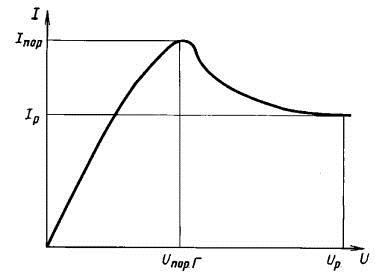
\includegraphics{рис5}
	\caption{Вольт-амперная характеристика диода Ганна}
	\label{fig:5}
\end{figure}
\par
\textbf{Детектор СВЧ излучения}. В данном случае генератор (диод Ганна) тесно связан с резонатором. Изменение параметров резонатора в такой системе приводит к автодинному эффекту. При поглощении мощности СВЧ излучения парамагнитными частицами образца изменяется добротность резонатора, следовательно, и напряженность СВЧ поля в месте расположения диода. Это приводит к изменению падения напряжения на диоде Ганна, что позволяет регистрировать сигнал ЭПР, в каждый отдельный момент времени пропорциональный поглощаемой при ЭПР мощности (при условии, что остальные факторы, влияющие на добротность резонатора, неизменны). В результате на обмотках ВЧ-трансформатора, включенного последовательно с диодом Ганна, формируется напряжение с частотой, равной частоте модуляции магнитного поля, и амплитудой, пропорциональной производной от кривой поглощения СВЧ-сигнала. Снимаемый со вторичной обмотки ВЧ-трансформатора сигнал усиливается и поступает в блок регистрации. 
\par  
\textbf{Высокочастотная модуляция} статического магнитного поля $ H_0 $ используется для повышения отношения сигнал/шум. За счет переноса спектра сигнала (при ВЧ модуляции) в область высоких частот $ f $ добиваются уменьшения мощности шумов кристаллического детектора СВЧ-поля с частотной зависимостью $ 1/f $. Модуляция статического поля $ H_0 $ высокочастотным (100 кГц) магнитным полем с малой амплитудой приводит к амплитудной модуляции выходного сигнала с детектора с той же частотой:
\begin{equation}
	U(H_0 + H_m \cos{\omega_m t}) \approx U(H_0) + \frac{dU}{dH} \cdot H_m \cos{\omega_m t}.
\end{equation}
\par 
Если амплитуда ВЧ модуляции меньше ширины резонансной линии, то амплитуда детектируемого сигнала (на частоте $ \omega_m $) будет приблизительно пропорциональна наклону кривой поглощения $ U(H_0) $ в центральной точке модулирующего поля (рис. 6), а именно интервальному среднему функции $ U(H_0) $ в точке: $ a(t)=dU/dH \cdot H_m $ . В результате при сканировании по магнитному полю регистрируется не сама кривая поглощения, а ее первая производная по полю $ dU/dH $.
\par 
Для ВЧ-модуляции на внешней стороне пластин резонатора размещены плоские спиральные катушки (катушки Гельмгольца) так, что их ось сонаправлена с осью катушек электромагнита, обеспечивающих развертку магнитного поля $ H_0 $.
\begin{figure}
	\centering
	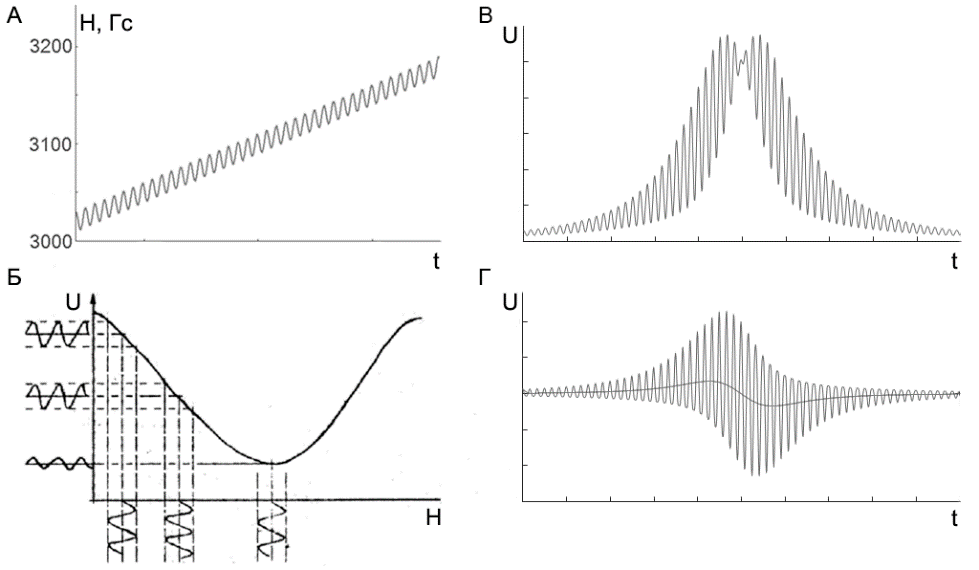
\includegraphics[scale=0.7]{рис6}
	\caption{Иллюстрация принципа ВЧ модуляции. А – изменение магнитного поля $ H_0 $ во времени с учетом развертки и ВЧ модуляции; Б – амплитуда $ a(t) $ детектируемого сигнала $ U(t)=a(t)\cos{\omega_m t} $ пропорциональна интервальному среднему кривой поглощения $ U(H_0) $; В – сигнал $ U(t) $, поступающий на вход синхронного детектора; Г – сигнал на выходе синхронного детектора, черная линия в центре – сигнал после фильтра нижних частот}
	\label{fig:6}
\end{figure}
\par 
\textbf{Синхронный детектор} - это устройство, осуществляющее перемножение входящих модулированного и опорного сигналов с учетом разности их фаз и последующую низкочастотную фильтрацию результата перемножения (рис. 6В, Г). 
\subsection{Форма линий в спектре ЭПР}
Интегральная интенсивность спектра ЭПР (площадь под кривой поглощения $ S $) при оптимальных условиях наблюдения пропорциональна количеству парамагнитных частиц. Численно значение площади под кривой линии поглощения можно получить либо дважды проинтегрировав полученный с ЭПР-спектрометра сигнал, либо по приближенной формуле:
\begin{equation}
	Y'_{max}(\Delta H_{max})^2 \sim S,
\end{equation}
где $ 2Y'_{max} $ - амплитуда между точками максимального наклона, $ \Delta H_{max} $ расстояние между экстремумами первой производной сигнала (рис.7).
\begin{figure}[h]
	\centering
	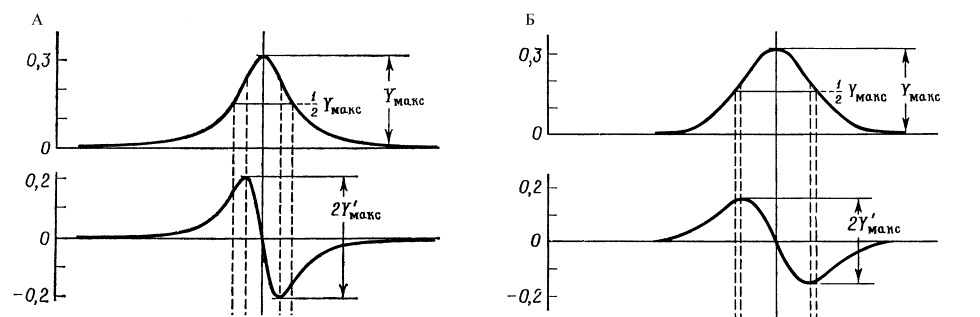
\includegraphics[width=0.7\linewidth]{рис7}
	\caption{Кривые поглощения и их первые производные в форме Лоренца (А) и Гаусса (Б)}
	\label{fig:7}
\end{figure}
\par
Соотношение между фактической шириной линии спектра на полувысоте $ \delta H_{max} $ и $ \Delta H_{max} $ зависит от формы линии спектра. Обычно в спектрах наблюдают две основные формы линии, которые описываются лоренцовым ($ y=a/(1+bx^2) $) или гауссовым ($ y=a \cdot \exp{-bx^2} $) контурами.
\par 
Для линии с лорецовым контуром связь между $ \delta H_{max} $ и $ \Delta H_{max} $ описывается соотношением
\begin{equation}
	 \Delta H_{max}  =\frac{2}{\sqrt{3}}  \delta H_{max} .
\end{equation}
Для линии с гауссовым контуром
\begin{equation}
	 \Delta H_{max} =\sqrt{\frac{2}{\ln{2}}}  \delta H_{max}. 
\end{equation}
\par
Форма линии спектра зависит от условий поглощения. Лоренцовы линии обычно наблюдают в спектрах ЭПР жидких растворов при низкой концентрации парамагнитных частиц. Если линия представляет собой суперпозицию многих линий (так называемая, неразрешенная сверхтонкая структура), то форма ее близка к гауссовой. Реальные линии ЭПР, как правило, в центральной части имеют форму, близкую к лоренцевой, по краям – к гауссовой.
\section{Ход работы}
Работа проводилась после прогрева спектрометра в течение не менее 20 мин, использовалась программа \textit{epr5g.exe}. Для контроля работы ЭПР-спектрометра был получен спектр ЭПР эталонного образца - дифенилпикрилгидразила (ДФПГ) концентрацией около 0.001 М, находящегося на конце фторопластового стержня, который вворачивается в полость резонатора.
\subsection{Исследование влияния амплитуды высокочастотной модуляции на вид спектров ЭПР}
Необходимо было зарегистрировать спектр ЭПР ДФПГ при нескольких амплитудах модуляции магнитного поля, которая определяется величиной тока в модуляционных катушках: от 0.05 до 1.80 А. Полученные спектры представлены на рис. 8. 
\begin{figure}[h]
	\centering
	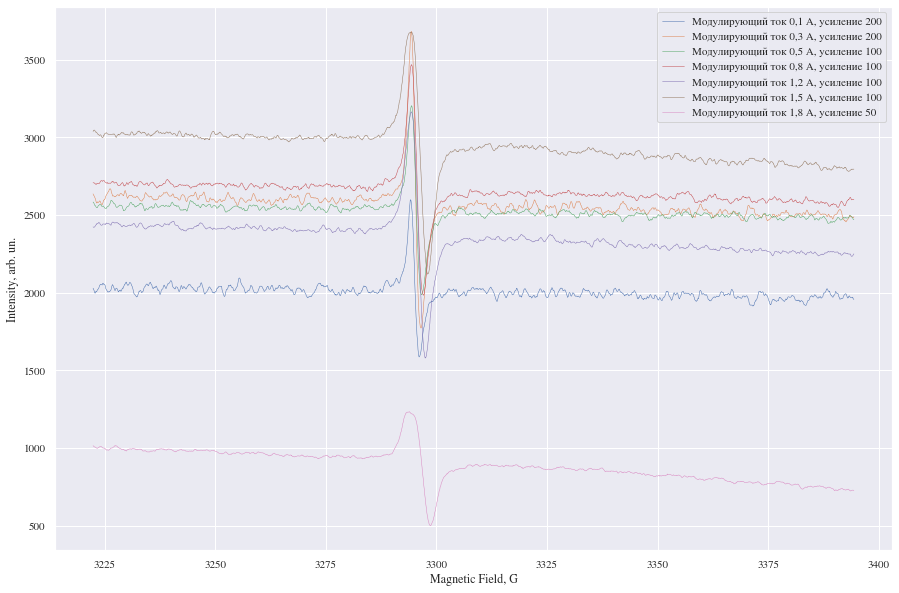
\includegraphics{рис8}
	\caption{ЭПР спектры ДФПГ при нескольких амплитудах модуляции магнитного поля}
	\label{fig:8}
\end{figure}
\par 
Форма кривой поглощения является лоренцовской, так как она характерна для жидких растворов с малой концентрацией парамагнитных частиц. По формуле (11) для спектра была рассчитана полуширина линии поглощения $ \delta H $ и была построена зависимость ширины от величины тока модуляции (рис. 9). Аппроксимация кривой была проведена методом наименьших квадратов, по наклону кривой была проведена оценка максимально достижимой для данного прибора амплитуды модуляции постоянного магнитного поля
\begin{gather*}
	H_{max} = (94 \pm 5) \cdot 10^{-2} \text{ Э}.
\end{gather*} 
\begin{figure}[h]
	\centering
	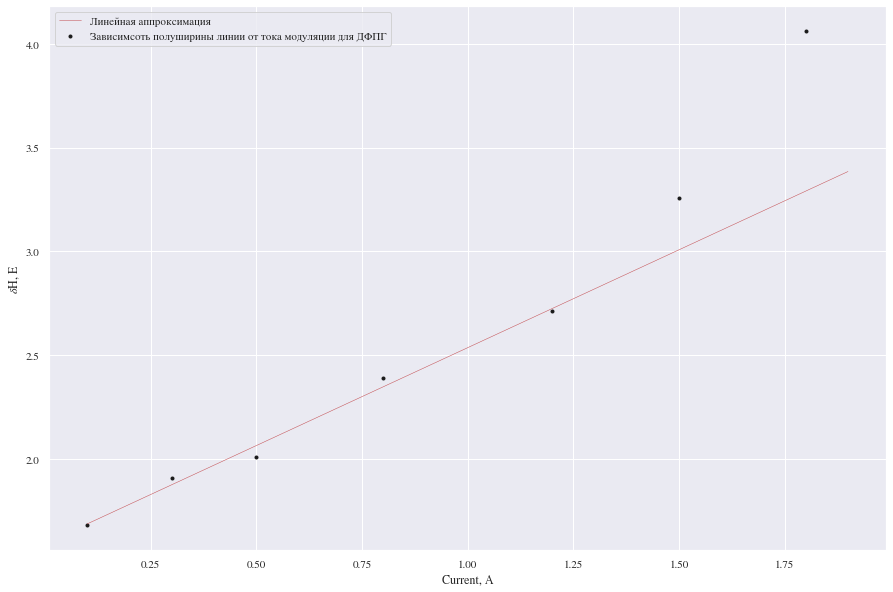
\includegraphics{рис9}
	\caption{Зависимость полуширины линии поглощения $ \delta H $ от величины тока модуляци для ЭПР спектров ДФПГ}
	\label{fig:9}
\end{figure}
\subsection{Исследование скорости спинового обмена в растворах и кристаллах}
Были зарегистрированы ЭПР спектры растворов соли $ \mathrm{Mn^{2+}} $ (концентрацией от 0.05 М до 0.8 М) (рис. 10). Форма кривой для спектров растворов с концентрацией 0.005 М и 0.1 М - лоренцова, для 0.5, 0.8, 1 М - гауссова. По формулам (11)-(12) была рассчитана полуширина линии поглощения $ \delta H $ и построена зависимость этой величины от концентрации (рис. 11). Угол наклона кривой был получен методом наименьших квадратов, из формулы (8) это величина
\begin{gather*}
	K_e/\gamma = 78 \pm 5 \text{ Э/М}.
\end{gather*}  
Тогда константа спинового обмена $ K_e $
\begin{gather*}
	K_e = (141 \pm 7) \cdot 10^7 \text{ 1/(M} \cdot\text{c)}.
\end{gather*}
Значения частоты столкновений парамагнитных частиц в растворах представлены в таблице 1.
\begin{table}[]
	\centering
	\begin{tabular}{|c|c|c|c|c|c|}
		\hline
		$C$, М             & 0.05          & 0.1        & 0.5            & 0.8         & 1                          \\ \hline
		$1/\tau_e, 10^7$ с & 7.1 $\pm$ 3.3 & 14 $\pm$ 7 & 70.7 $\pm$ 3.3 & 113 $\pm$ 5 & 141 $\pm$ 7 \\ \hline
	\end{tabular}
\caption{Значения частоты столкновений парамагнитных частиц в растворах}
\end{table}
\begin{figure}[h]
	\centering
	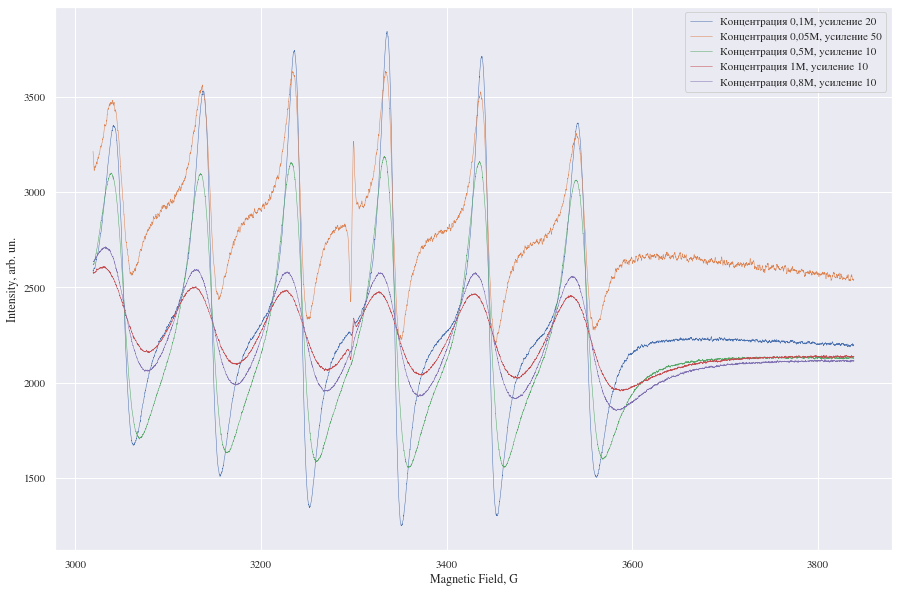
\includegraphics{рис10}
	\caption{ЭПР спектры растворов соли $ \mathrm{Mn^{2+}} $ с разными концентрациями}
	\label{fig:10}
\end{figure}
\begin{figure}[h]
	\centering
	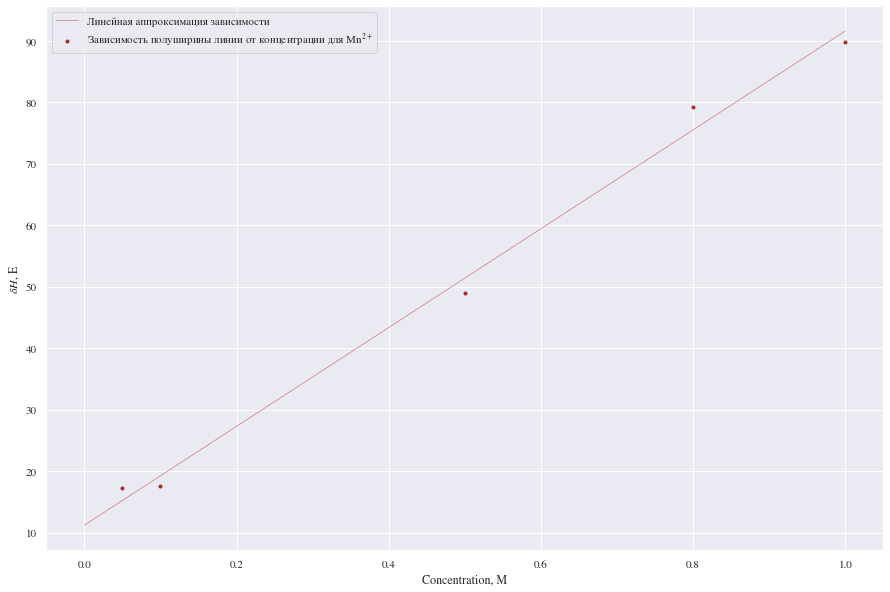
\includegraphics{рис11}
	\caption{Зависимость полуширины линии поглощения $ \delta H $ ЭПР спектра раствора соли $ \mathrm{Mn^{2+}} $ от концентрации}
	\label{fig:11}
\end{figure}
\par 
По формуле (10) для каждого раствора была рассчитана интегральная интенсивность спектра ЭПР $ S $ и был построен график зависимости $ S $ от концентрации раствора (рис. 12). Измерения проводились на крайнем левом пике, поскольку перекрытие с соседними пиками для него наименьшее. 
\begin{figure}[h]
	\centering
	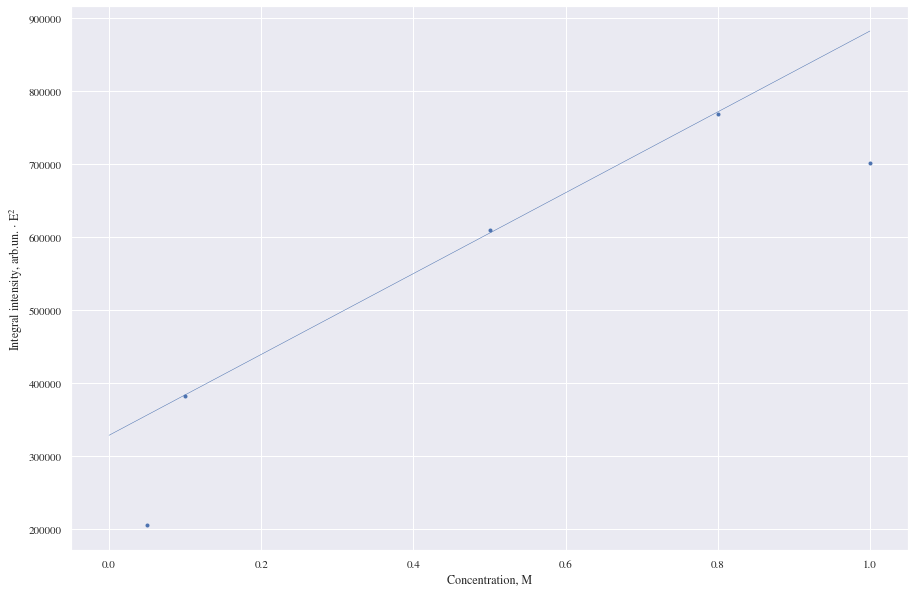
\includegraphics{рис12}
	\caption{График зависимости интегральной интенсивности спектра ЭПР от концентрации раствора}
	\label{fig:12}
\end{figure}
\par 
Далее был зарегистрирован спектр порошка соли $ \mathrm{Mn^{2+}} $ в сухой пробирке (рис. 13). При качественном сравнении спектров ЭПР соли $ \mathrm{Mn^{2+}} $ в растворе и в кристаллическом состоянии можно сделать вывод, что в растворе наблюдается медленное спиновое взаимодействие, а в кристаллическом состоянии - быстрое, так как в спектре при этом наблюдается только одна линия резонанса - на средней частоте. Также резонансные линии в спектре являются более узкими, что говорит об обменном сужении. 
\begin{figure}
	\centering
	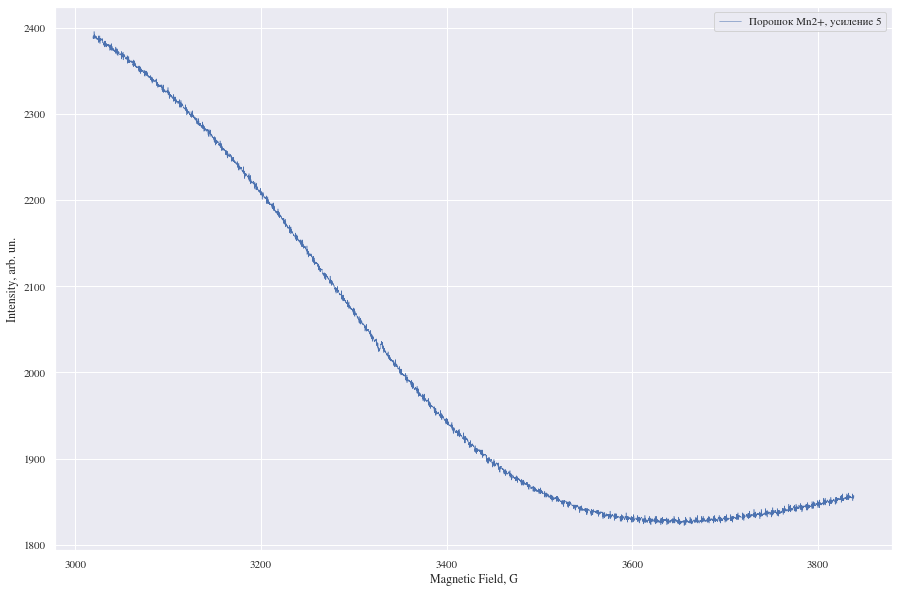
\includegraphics{рис13}
	\caption{Спектр ЭПР порошка соли $ \mathrm{Mn^{2+}} $}
	\label{fig:13}
\end{figure}
\subsection{Исследование сверхтонкой структуры спектров ЭПР}
Из свойства эквидистантности линий ЭПР была определена константа сверхтонкого взаимодействия:
\begin{gather*}
	a=100\pm 5 \text{ Э.}
\end{gather*}
Спин ядра для ионов $ \mathrm{Mn^{2+}} $ - 5/2, значением спина определяется число линий в спектре ЭПР - 6. Для расщепления линий в спектре под влиянием парамагнитных ядер одиночных атомов интенсивности линий в спектре одинаковые. 
\par
Также был снят спектр порошка мела (рис. 14). На графике можно увидеть 6 линий поглощения, причиной этому является ядро со спином 5/2. У иона кальция спин ядра - 7/2, что соответствовало бы 8 линиям в спектре. Это связано с наличием ионов $ \mathrm{Mn^{2+}} $, так как в природе ионы кальция всегда идут в паре с ионами марганца.
\begin{figure}[h]
	\centering
	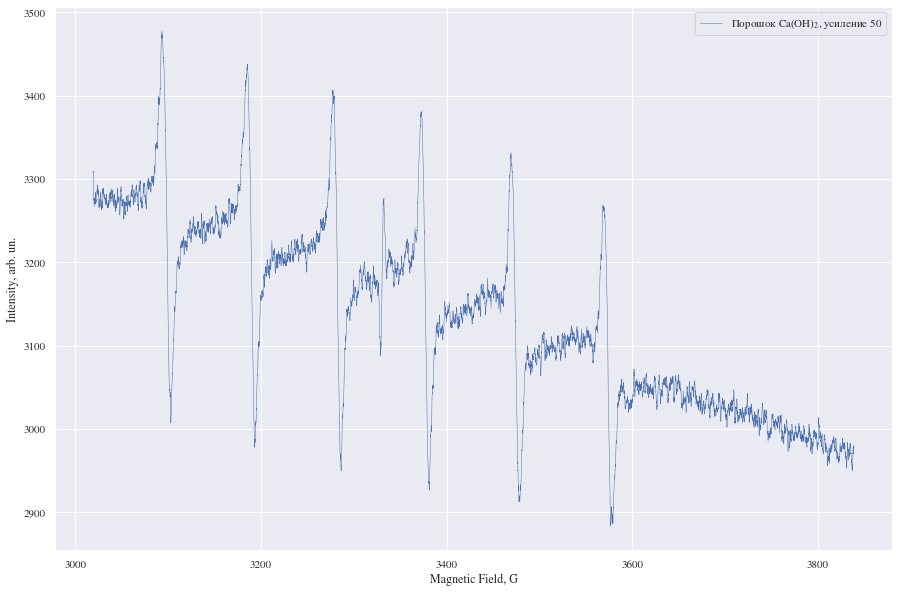
\includegraphics{рис14}
	\caption{Спектр порошка мела}
	\label{fig:14}
\end{figure}
\subsection{Исследование влияния уровня диэлектрических потерь на вид спектров ЭПР}
Для раствора низкой концентрации был снят спектр 
\begin{enumerate}
	\item в капилляре;
	\item в пробирке, сохраняя ту же высоту столба жидкости, что и в пунте 1;
	\item в пробирке, сохраняя то же количество парамагнитных центров, что и в пункте 1 при таком же объеме, как в пункте 2. 
\end{enumerate}
\begin{figure}[h]
	\centering
	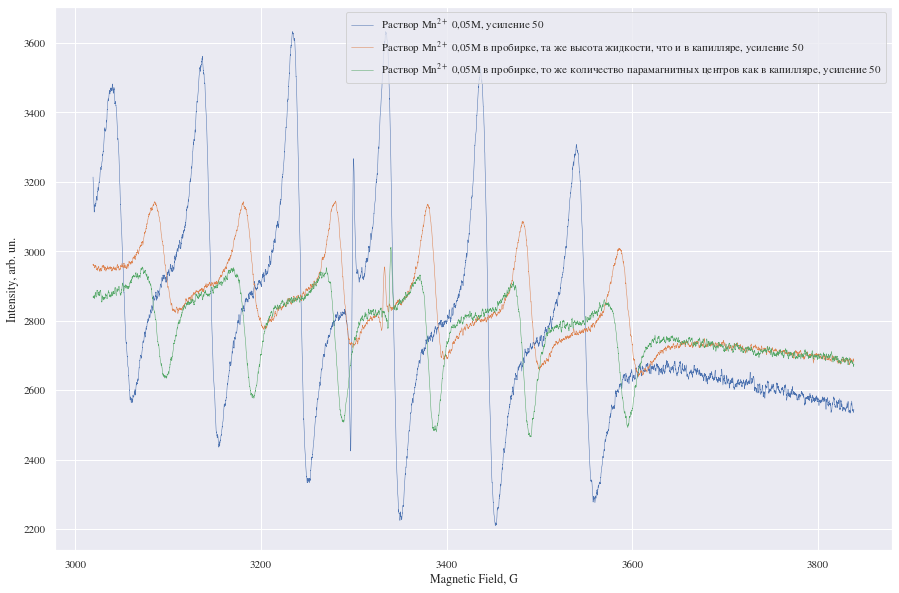
\includegraphics{рис15}
	\caption{Спектр ЭПР для разного уровня диэлектрических потерь}
	\label{fig:15}
\end{figure}
\par
Для спектра из пункта 1 наблюдается наибольшая амплитуда сигнала, наименьшая ширина пика и более четкий сигнал. Далее, так как в пункте 2 объём образца увеличился, диэлектрические потери увеличились, что привело к уменьшению амплитуды сигнала и сдвигу линий поглощения, так как неоднородность магнитного поля увеличилась. В пункте 3 количество парамагнитных центров уменьшилось по сравнению с пунктом 2, поэтому уменьшилось поглощение и, соответственно, амплитуда сигнала. 
\par 
Оценку уровней диэлектрических потерь в растворе можно проводить путём сравнения амплитуд сигналов в спектре.
\subsection{Исследование формы линий} 
Для растворов низких концентраций форма линии поглощения лучше описывается лоренцовским контуром, а для растворов более высокой концентрации - гауссовым контуром. Форма линий спектра зависит от условий поглощения. Лоренцовский контур наблюдается при низкой концентрации параманитных частиц, гауссов - когда линия представляет собой суперпозицию многих линий. Полученные линии ЭПР в центральной части имеют форму, близкую к лоренцовой, по краям - к гауссовой.
\section{Выводы:}
\begin{enumerate}
	\item Был зарегистрирован спектр эталонного образца - ДФПГ, концентрацией около 0.001 М при разных амплитудах модуляции. С увеличением амплитуды модуляции ширина линии увеличивается. Была проведена оценка максимально достижимой для данного прибора амплитуды модуляции постоянного магнитного поля, в результате
	\begin{gather*}
		H_{max} = (94 \pm 5) \cdot 10^{-2} \text{ Э}.
	\end{gather*} 
	\item Были зарегистрированы ЭПР спектры растворов соли $ \mathrm{Mn^{2+}} $ при низких и высоких концентрациях. Для каждого случая была определена полуширина линии поглощения и построена зависимость этой величиной от концентрации. В результате удалось определить константу спинового обмена 
	\begin{gather*}
		K_e = (141 \pm 7 \cdot 10^7 \text{ 1/(M} \cdot\text{c)}
	\end{gather*}
	и значения частоты столкновений парамагнитных частиц в растворе (таблица 1).
	\item 
	Был снят спектр порошка соли иона марганца. При сравнении спектров растворов и порошка соли $ \mathrm{Mn^{2+}} $ был сделан вывод, что в растворе наблюдается медленное спиновое взаимодействие, а в кристаллическом состоянии - быстрое.
	\item 
	Также был проведён визуальный анализ формы линий поглощения. Было выявлено, что при низких концентрация форма линии лучше соответствует лоренцовской кривой, а для растворов более высокой концентрации - гауссовой, что подтверждает теорию.
	\item
	Проведено исследование сверхтонкой структуры спектров ЭПР для ионов $ \mathrm{Mn^{2+}} $ и определена константа сверхтонкого взаимодействия 
	\begin{gather*}
		a=100\pm 5 \text{ Э.}
	\end{gather*}
	\item 
	Исследовано влияние объёма образца и концентрации парамагнитный центров на диэлектрические потери при снятии спектра. В результате был подтвержден экспериментально теоретический факт: при меньшем объёме образца меньше диэлектрические потери при снятии спектра.
\end{enumerate}
\end{document}
